\documentclass[acmtog]{acmart}
\settopmatter{printacmref = false}
\settopmatter{printccs = false}
\settopmatter{printfolios = false}
\renewcommand\footnotetextcopyrightpermission[1]{}
\pagestyle{plain}
\acmJournal{TOG}

\begin{document}

%%
%% The "title" command has an optional parameter,
%% allowing the author to define a "short title" to be used in page headers.
\title{Advanced Computer Graphics Final Report}

%%
%% The "author" command and its associated commands are used to define
%% the authors and their affiliations.
%% Of note is the shared affiliation of the first two authors, and the
%% "authornote" and "authornotemark" commands
%% used to denote shared contribution to the research.
\author{Jingyi Lyu}
\email{lv-jy22@mails.tsinghua.edu.cn}
\affiliation{%
	\institution{2022010874}
	\country{CS23, IIIS}
}

%%
%% This command processes the author and affiliation and title
%% information and builds the first part of the formatted document.
\maketitle

\section{Introduction}
For the final project of advanced computer graphics course this semester, my team have chosen project topic \verb|Image Rendering| and implemented a basic physically-based renderer which runs on software pipeline. My teammate is Shengquan Du from CS21 of IIIS.

We have accomplished a bunch of functions and materials, following the instruction of project topic provided. Precisely, we have implemented:

\begin{itemize}
	\item A path tracing algorithm handling diffusive (Lambertian) and specular material.
	\item Acceleration structure based on BVH.
	\item Transmissive material.
	\item Customized material based on principled BSDF.
	\item Color texture and normal texture. 
	\item Anti-aliasing.
	\item Importance sampling and multiple importance sampling.
	\item Volumetric rendering effects, including homogeneous and inhomogeneous volume rendering, channel independent subsurface scattering, volumetric emission and volumetric alpha shadow. 
	\item Special visual effects: Motion blur and depth of field based on trivial aperture.
	\item A self-made complicated scene.
\end{itemize}

Our implementation did not start from scratch, but developed from the \verb|sparkium| framework provided by TAs. For technical issues, we mainly refer to the web version of \textit{Physically Based Rendering: From Theory To Implementation} \cite{pbr3rd} and the corresponding codebase \verb|pbrt-v3| \cite{pbrt}. Our own codebase can be found at \url{https://github.com/qwaszx-D/sparkium}.

Results of those finished tasks is presented in detail below.

\section{Basic Functions}

A typical path tracing algorithm handling diffusive and specular material was implemented first. We applied it to the popular test scene \verb|Cornell Box|, with result shown in \ref{cornell128} and \ref{cornell_specular}.

\begin{figure}[h]
	\centering
	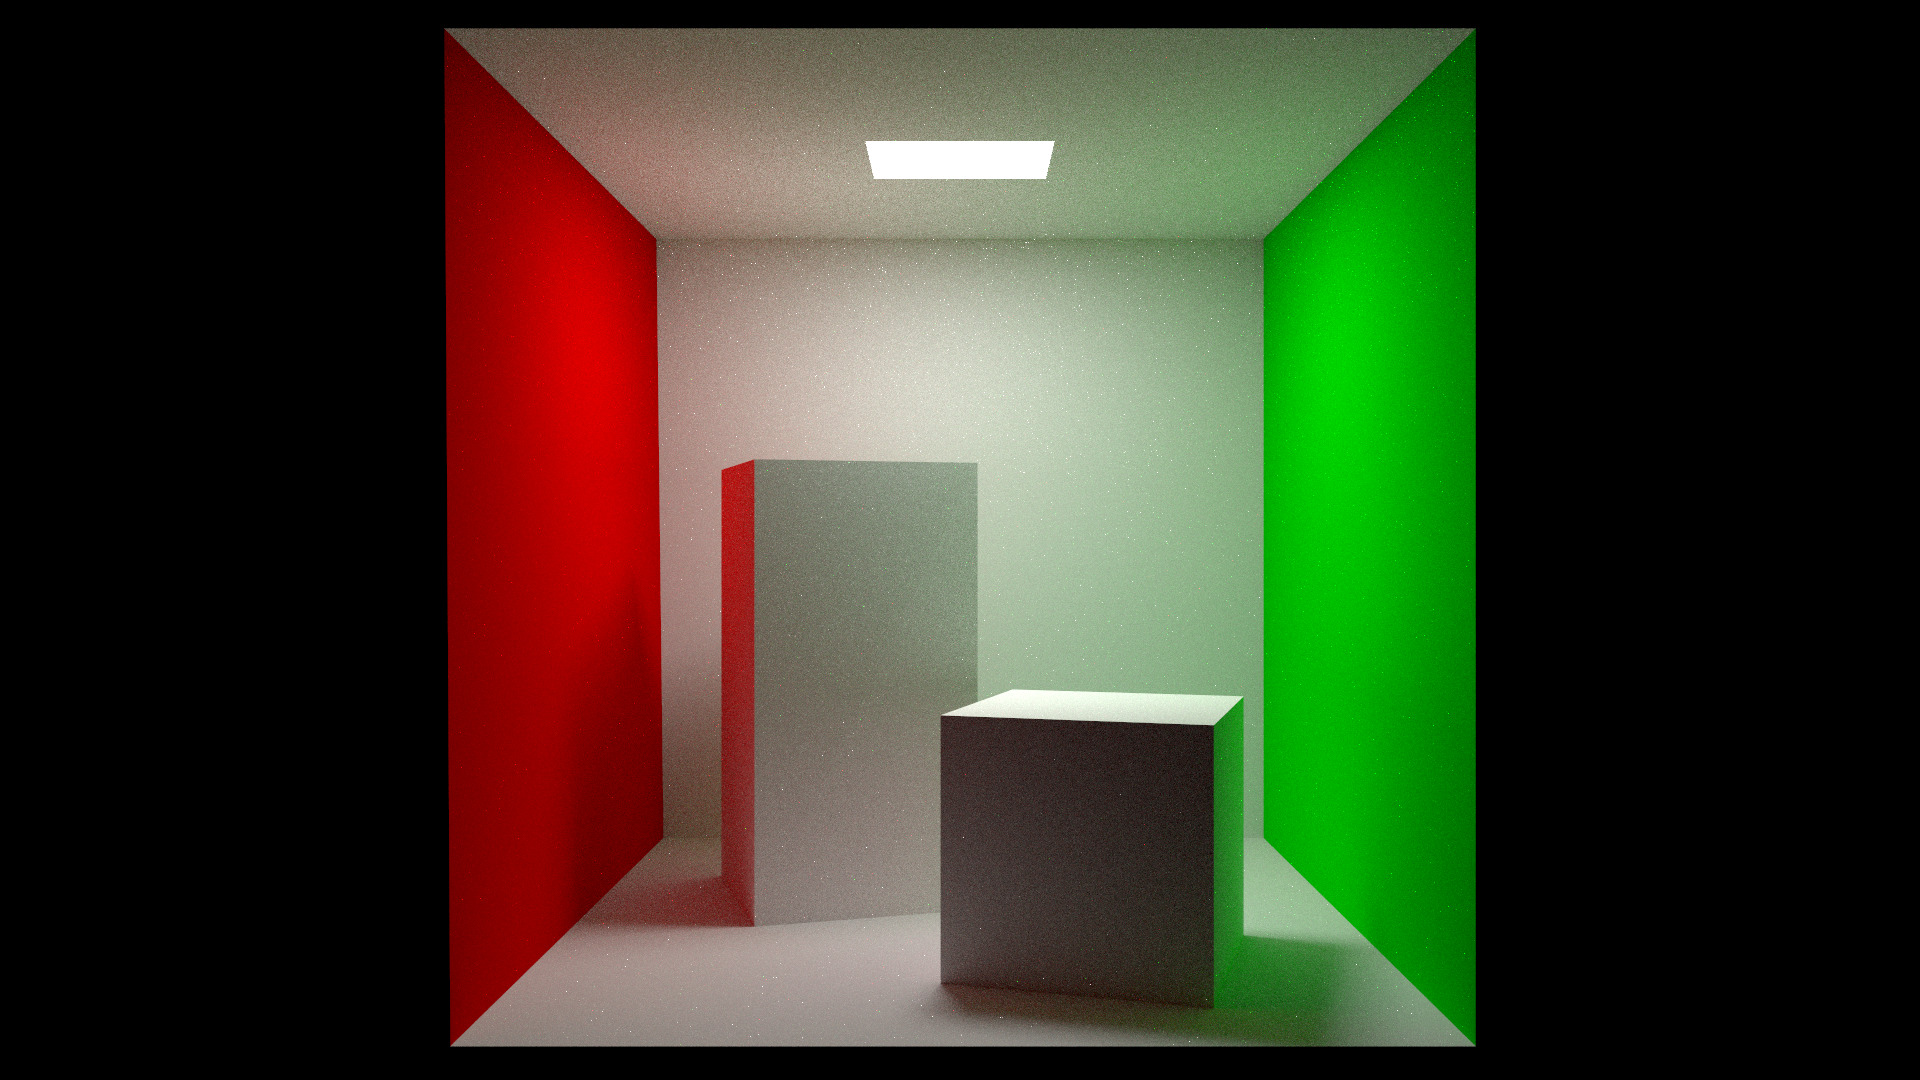
\includegraphics[width=\linewidth]{cornell128}
	\caption{Cornell Box}
	\label{cornell128}
\end{figure}

\begin{figure}[h]
	\centering
	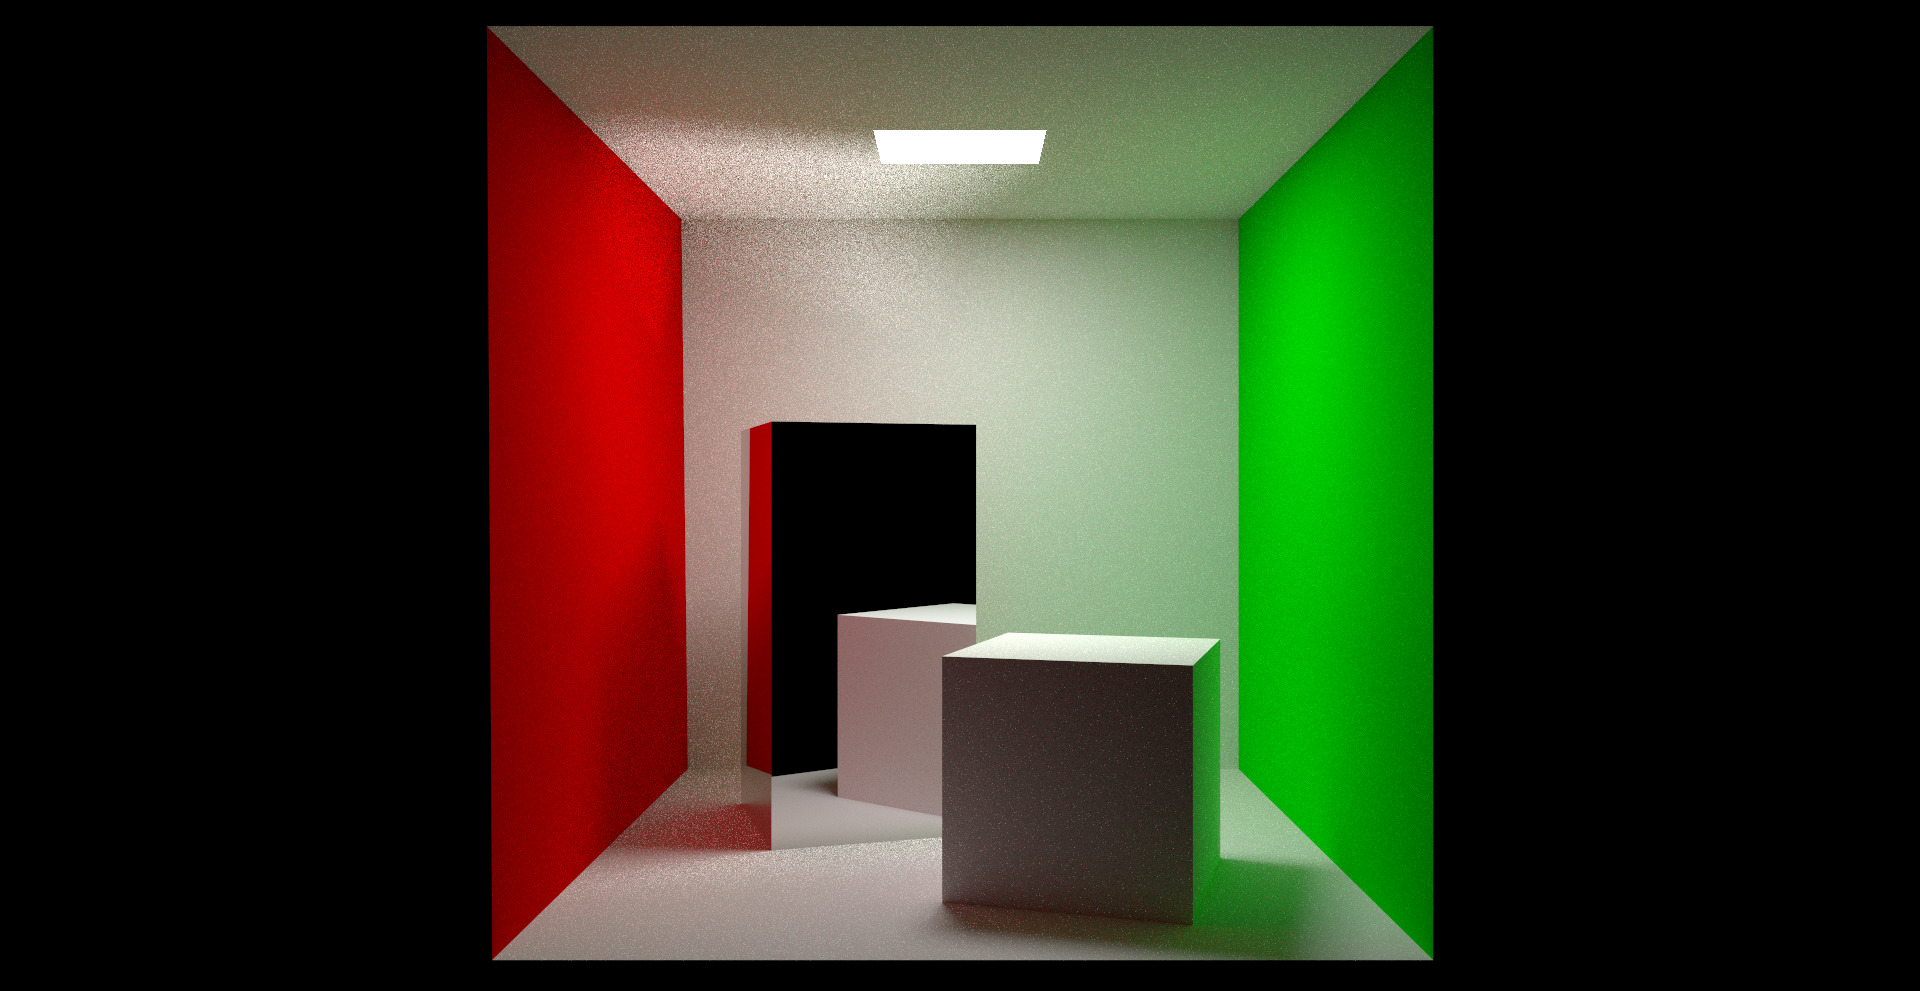
\includegraphics[width=\linewidth]{cornell_specular}
	\caption{Cornell Box with specular material}
	\label{cornell_specular}
\end{figure}

\noindent \textbf{Contribution}: Jingyi Lyu. 

\section{Advanced Materials}

\subsection{Transmissive Material}

Specular transmissive material was implemented and resulted in \ref{cornell_transmissive}. The bottom part of block is dim because the floor under block cannot receive direct illumination (since we did not implemented alpha shadow for this case). The ``block" actually does not have bottom face, which maybe also a reason.

\noindent \textbf{Contribution}: Shengquan Du.

\begin{figure}[h]
	\centering	
	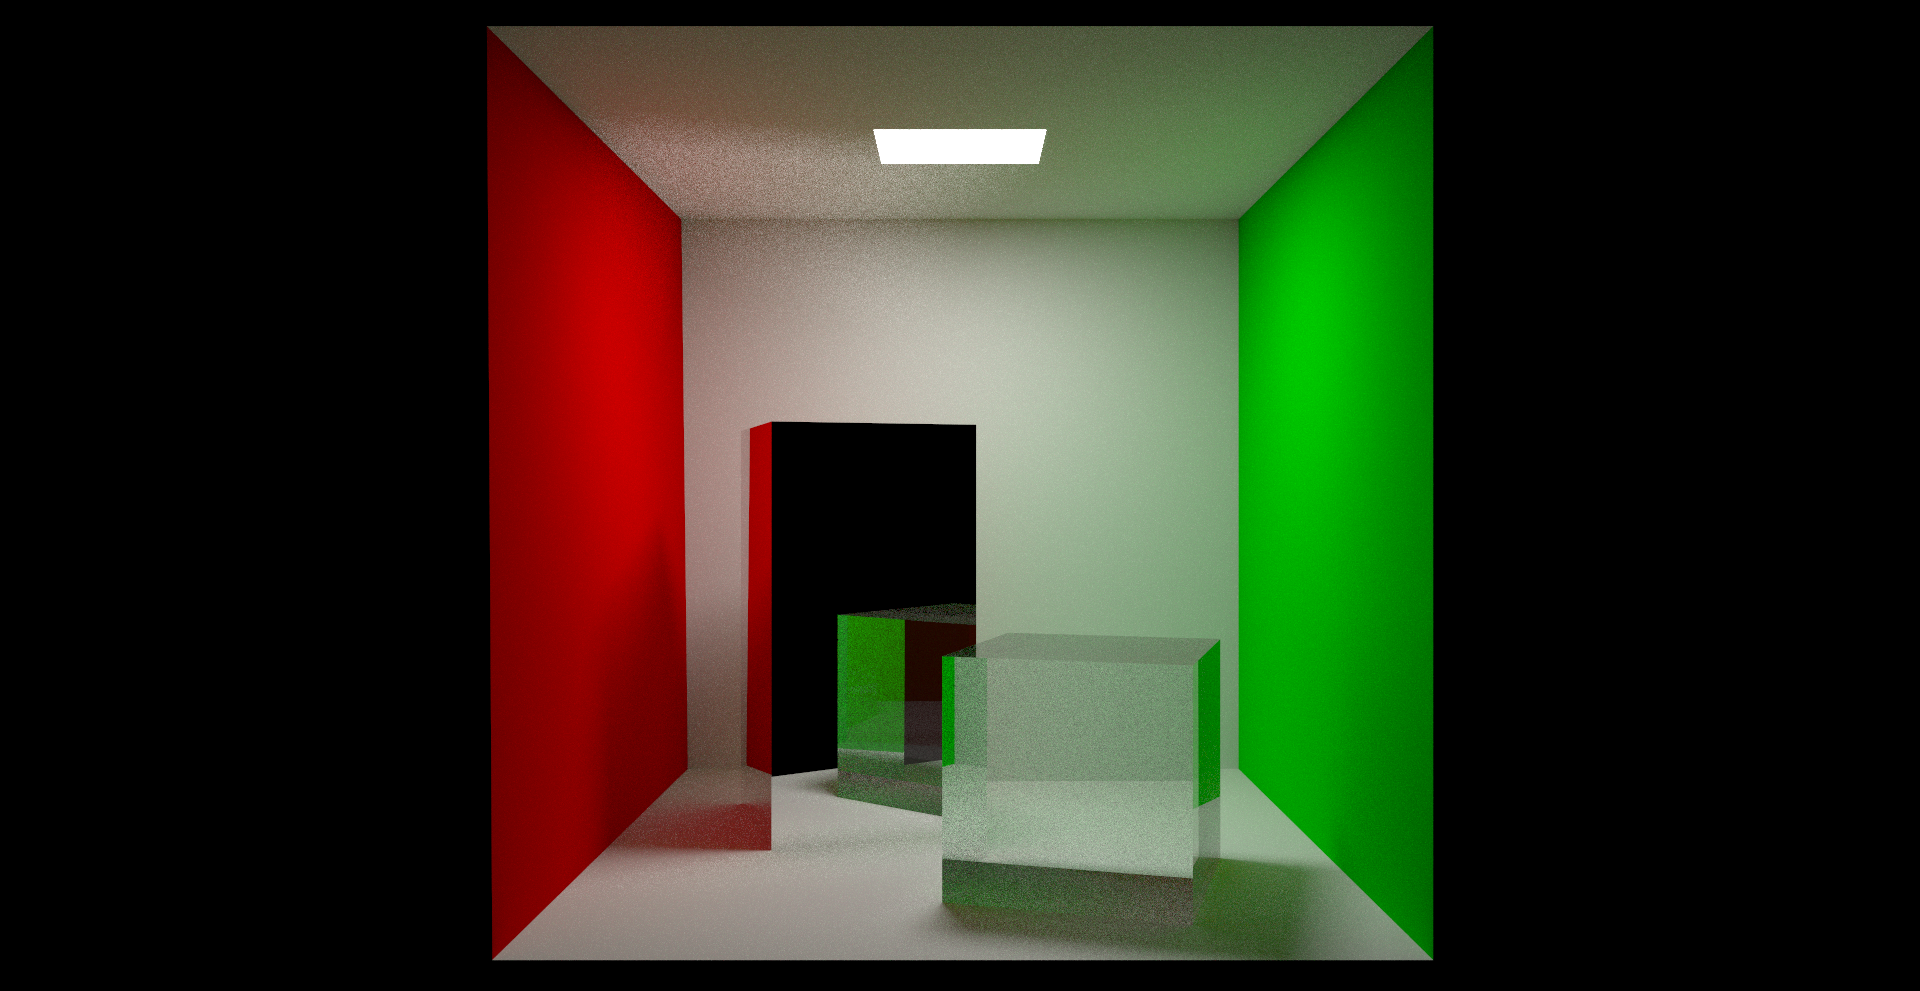
\includegraphics[width=\linewidth]{cornell_transmissive}
	\caption{Cornell Box with transmissive material}
	\label{cornell_transmissive}
\end{figure}

\subsection{Principled BSDF}

Complicated customized material based on Disney Principled BSDF was implemented. A fancy result is shown in \ref{sea}, where the sea surface is made of principled BSDF with parameter Albedo = [0.064 0.130 0.292], Eta = 1.33, Metallic = 0.8, Roughness = 0.1, Alpha = 0.925, Transmission = 1. 

\begin{figure}[h]
	\centering	
	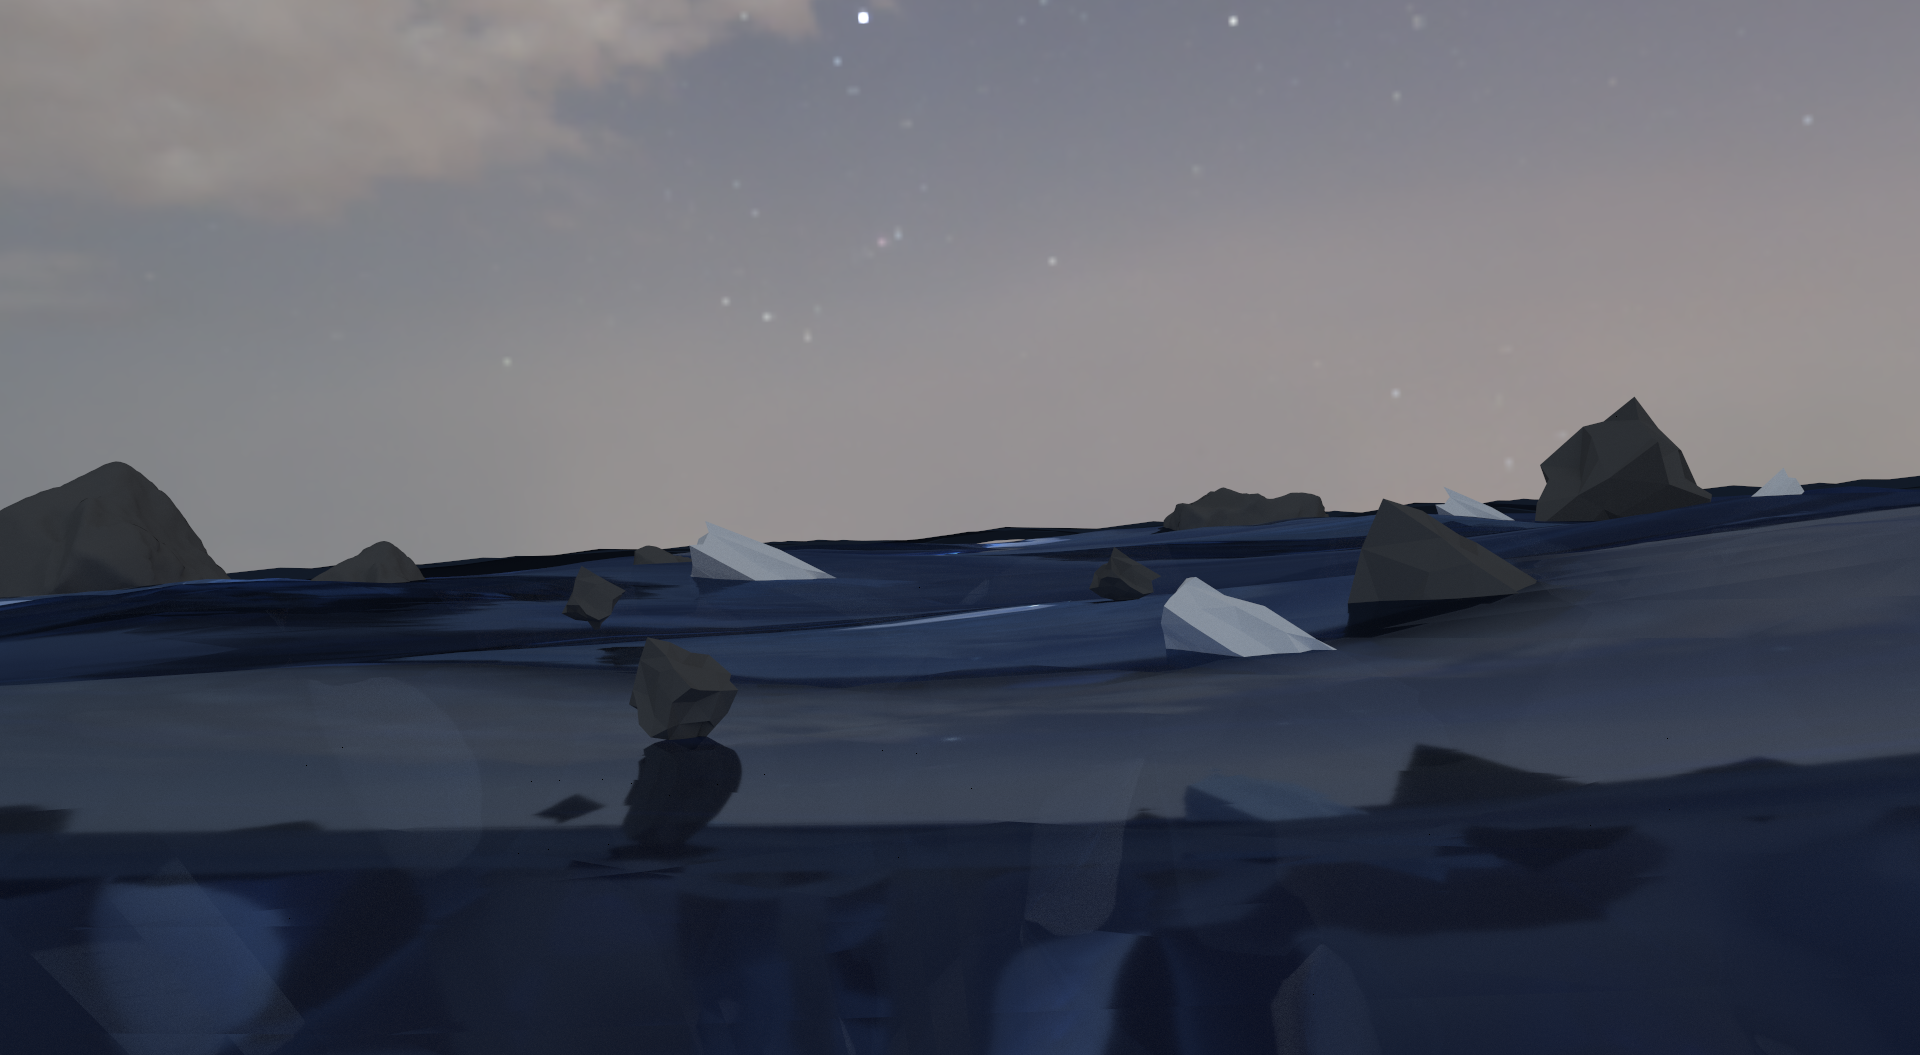
\includegraphics[width=\linewidth]{sea}
	\caption{Cornell Box with transmissive material}
	\label{sea}
\end{figure}

\noindent \textbf{Contribution}: Shengquan Du.

\subsection{Volumetric Rendering}

We have implemented volumetric rendering effects based on volumetric light transport and bidirectional subsurface scattering reflection distribution function (BSSRDF) respectively, whitch has covered most requirements of this course project.

Volumetric light transport is similar to normal path tracing, but light has probability interacting with participating medium which proportional to attenuation coefficient of medium. Upon interaction, an incident direction is sampled according to phase function, which defines the angular distribution of scattered radiation at a point. Based on travelling distance and attenuation strength, the proportion of reduce in light (as well as shadow ray, when estimating direct illumination) strength can be computed. 

BSSRDF is a fast approximation to true volumetric scattering. It is usually presented in form of $S(p_o, w_o, p_i, w_i)$, which is extened from $BSDF$ by adding degree of freedom about incident position $p_i$. The property of BSSRDF materials are determined by parameters including albedo, mean free path length and refractive index. 

One can refer to Chapter 11 and Chapter 15 of \cite{pbr3rd} for detail.

\noindent \textbf{Contribution}: Jingyi Lyu.

\subsubsection{Volumetric Light And Fog (Volumetric Light Transport)}

As typical volumetric rendering effect, we have implemented homogeneous volumetric light and volumetric fog, shown in \ref{vol_light} and \ref{heavy_fog}.

\begin{figure}[h]
	\centering	
	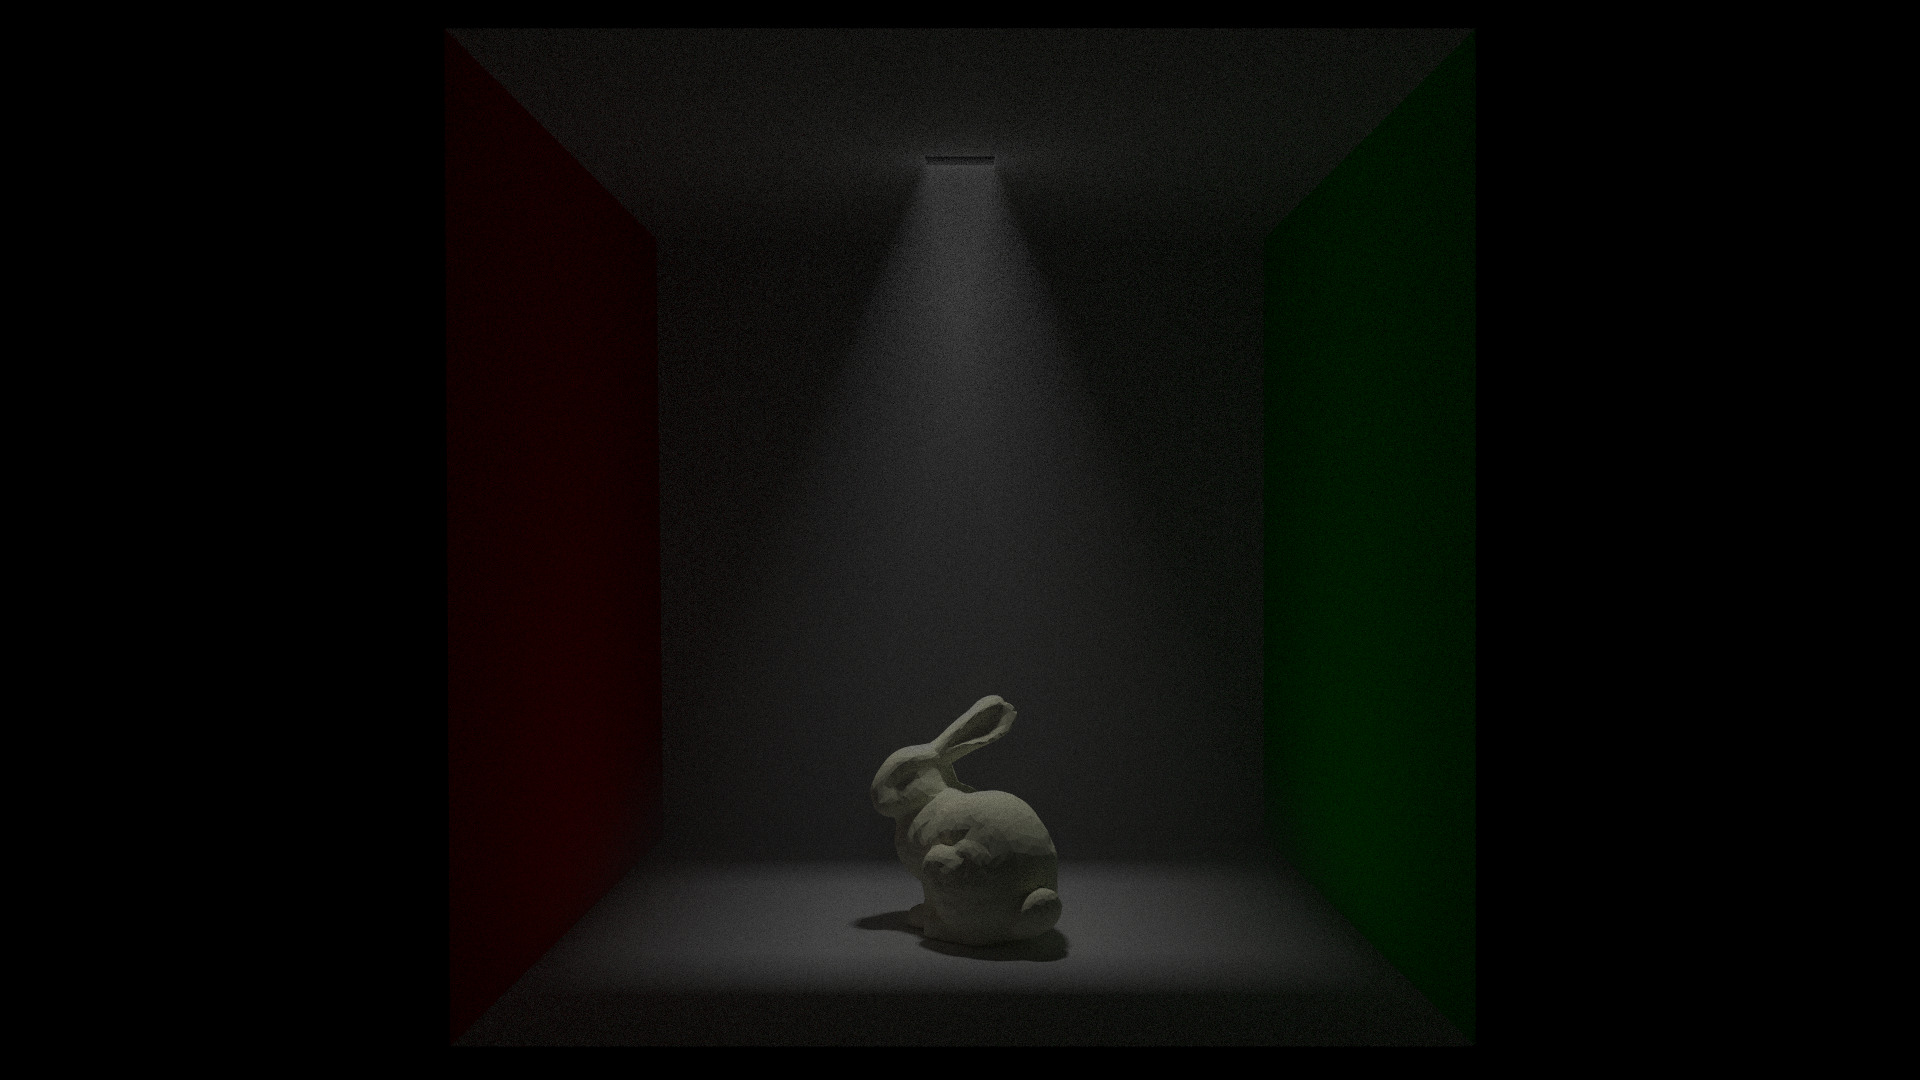
\includegraphics[width=\linewidth]{vol_light}
	\caption{Volumetric light in dim space}
	\label{vol_light}
\end{figure}

\begin{figure}[h]
	\centering	
	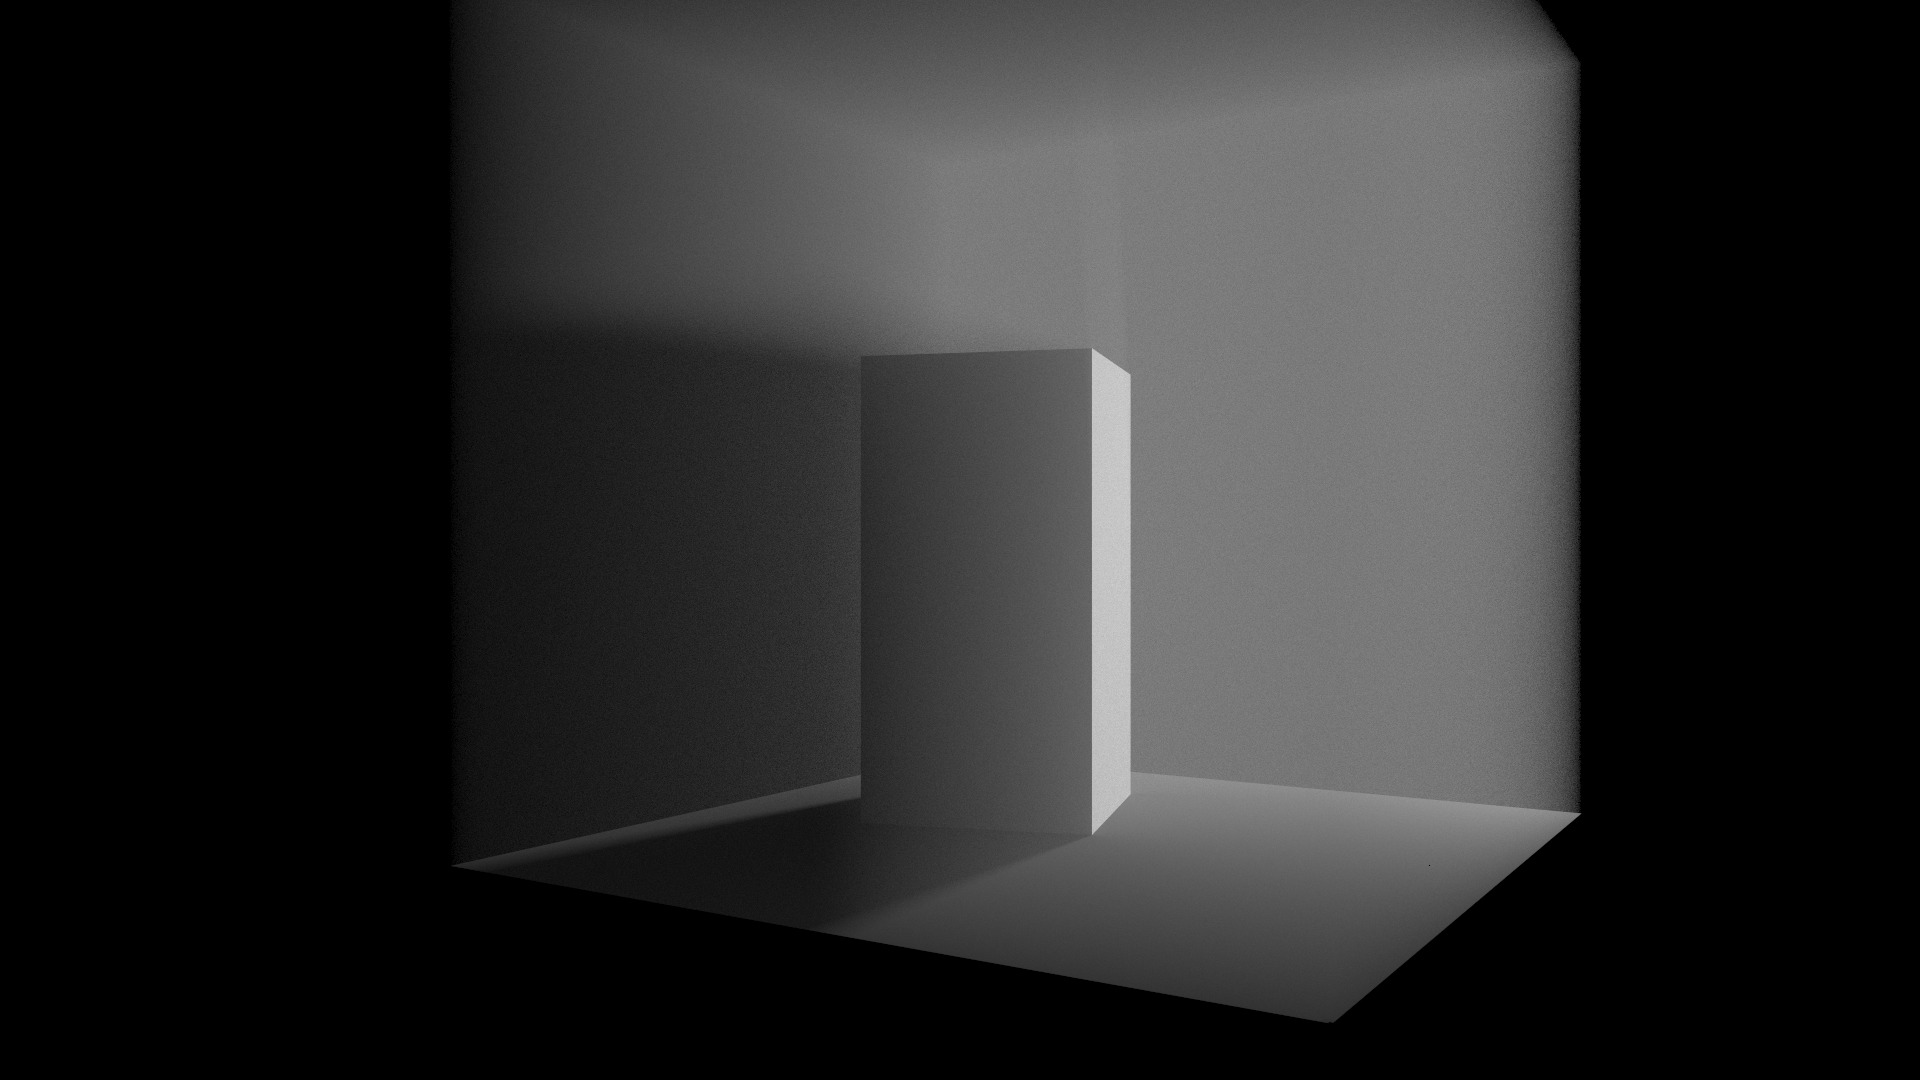
\includegraphics[width=\linewidth]{heavy_fog}
	\caption{Heavy fog illuminated by strong light source}
	\label{heavy_fog}
\end{figure}

\subsubsection{Inhomogeneous Volumetric Medium (Volumetric Light Transport)}

We provided support for inhomogeneous medium whose density varies throught the space. Density grid is required to express those medium, which is stored in external file and read at each loading. To sample medium with varying density correctly, we used delta tracking. The result is shown in \ref{inhomo_vol}.

\begin{figure}[h]
	\centering	
	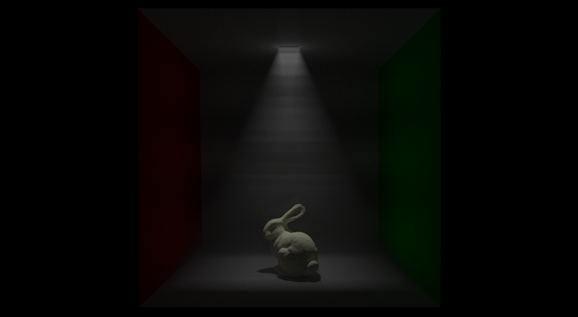
\includegraphics[width=\linewidth]{inhomo_vol}
	\caption{Volumetric light in inhomogeneous medium}
	\label{inhomo_vol}
\end{figure}

\subsubsection{Volumetric Emission (Volumetric Light Transport)}

Volumetric emission effect is shown in \ref{vol_emission}. We did not provide importance sampling support for this.

\begin{figure}[h]
	\centering	
	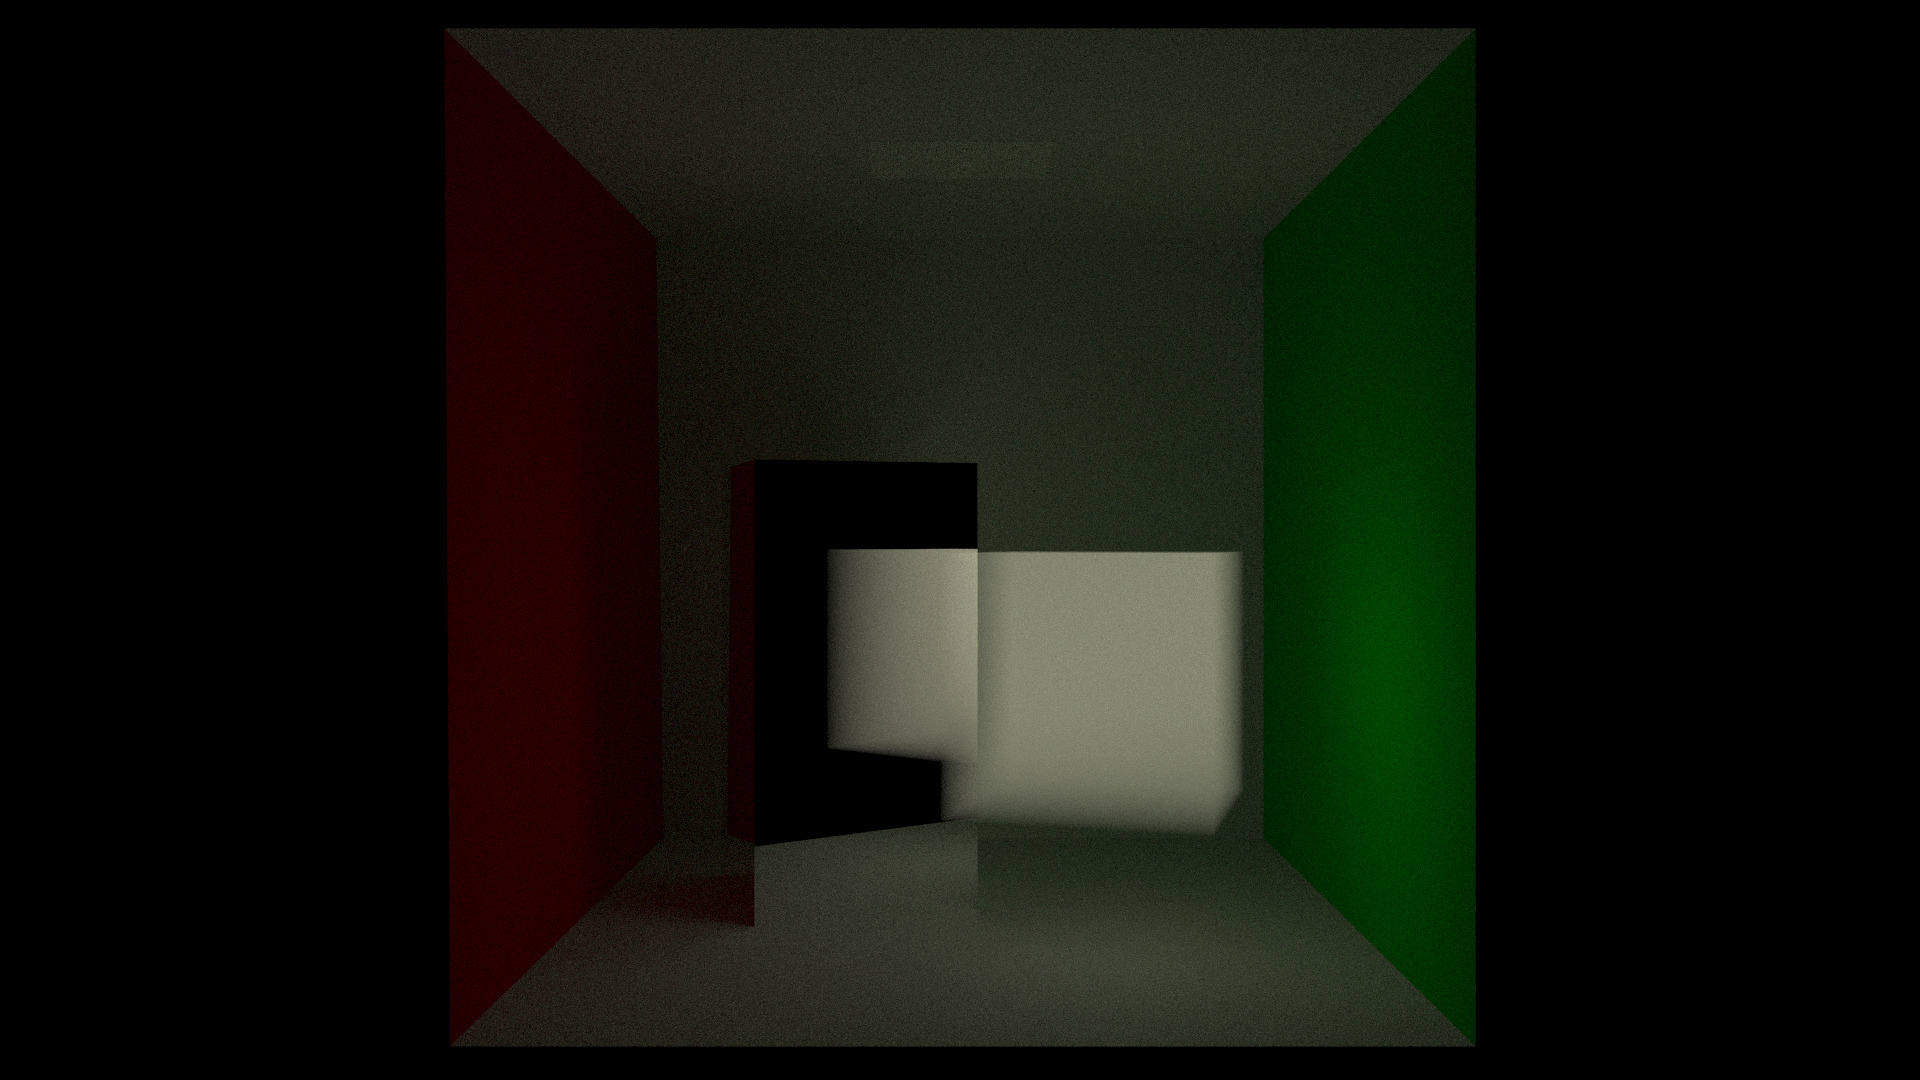
\includegraphics[width=\linewidth]{vol_emission}
	\caption{Volumetric emission}
	\label{vol_emission}
\end{figure}

\subsubsection{Volumetric Alpha Shadow (Volumetric Light Transport)}

Attenuation of shadow ray elicits volumetric alpha shadow. Based on different estimation mechanism of attenuation in homogeneous and inhomogeneous case, our alpha shadow also supports homogeneous and inhomogeneous case, which are shown in \ref{vol_alpha_homo} and \ref{vol_alpha_inhomo}. In the latter scene, the fog on left side is slightly denser than right side, so as the shadow. Some patterned texture appears on the fog due to pseudo random feature or floating point error during grid generation and scattering sampling.

\begin{figure}[h]
	\centering	
	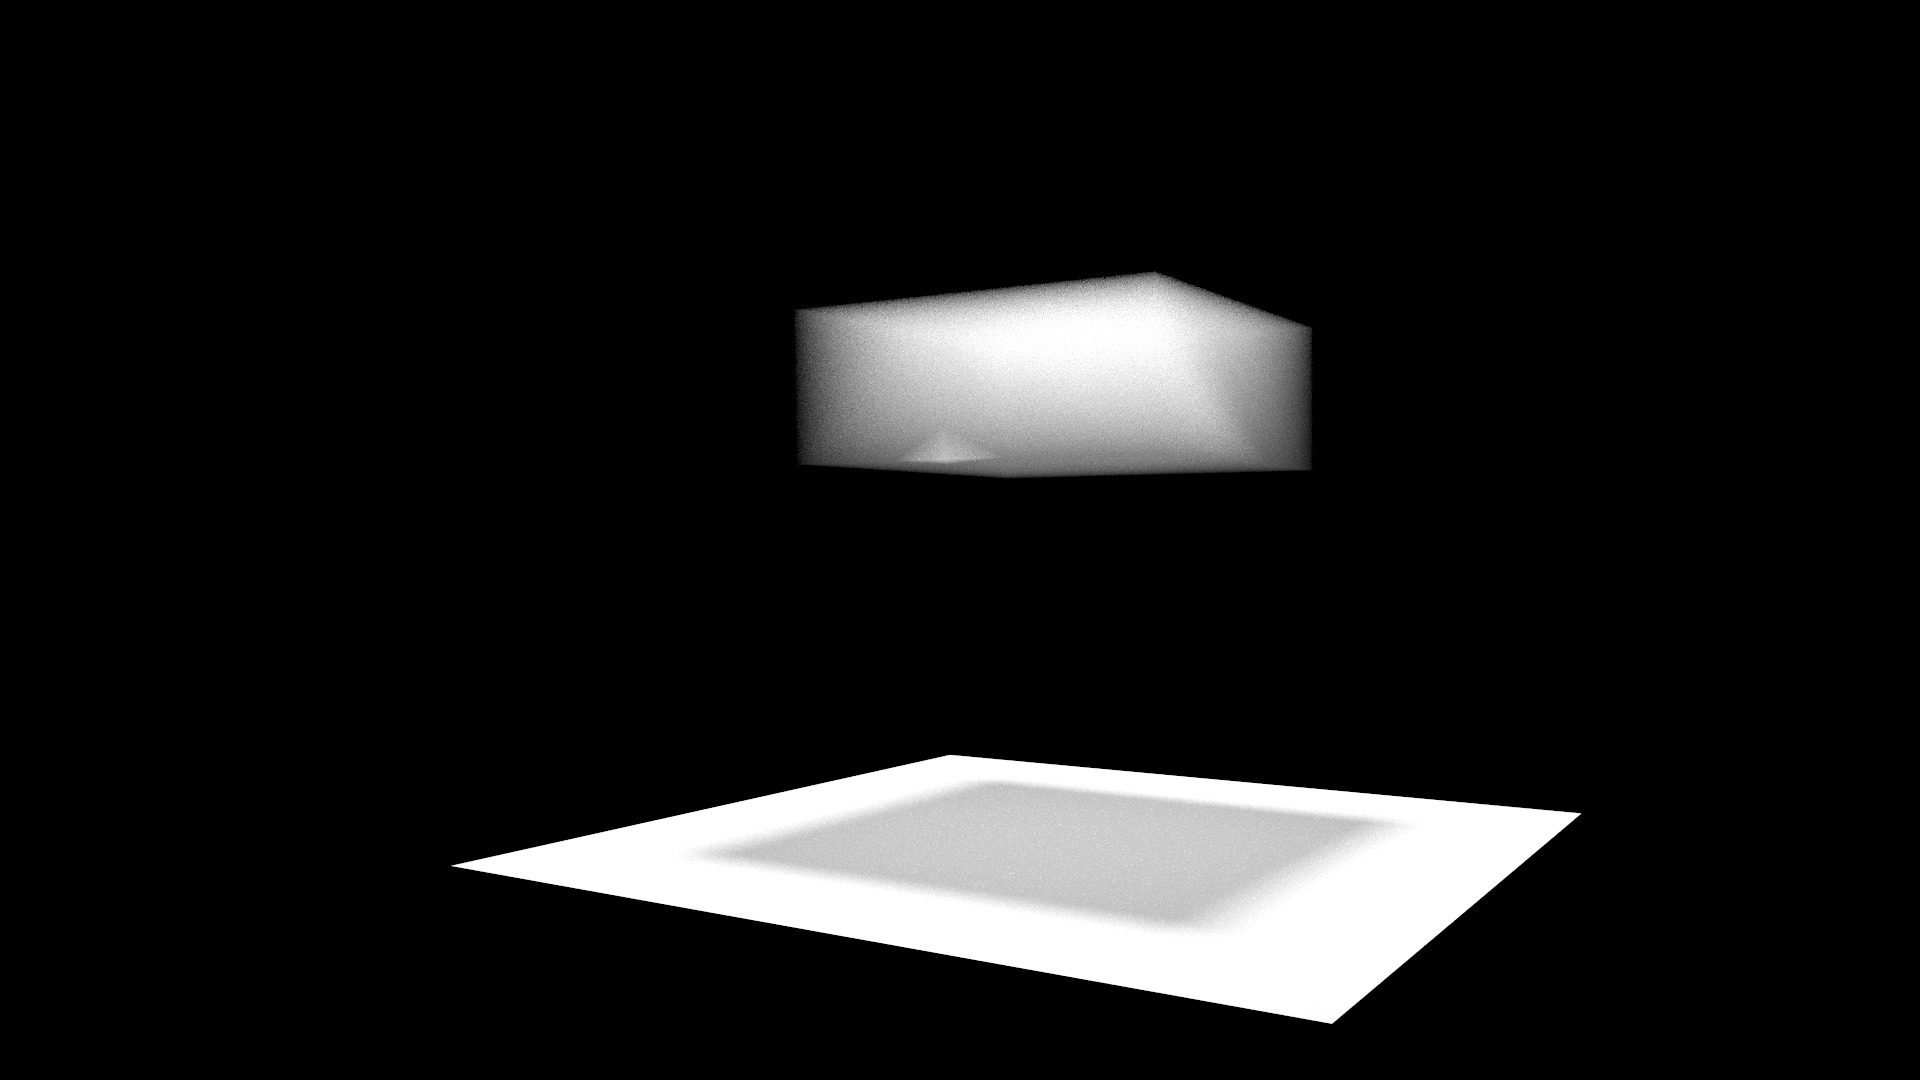
\includegraphics[width=\linewidth]{vol_shadow_homo}
	\caption{Homogeneous volumetric alpha shadow}
	\label{vol_alpha_homo}
\end{figure}

\begin{figure}[h]
	\centering	
	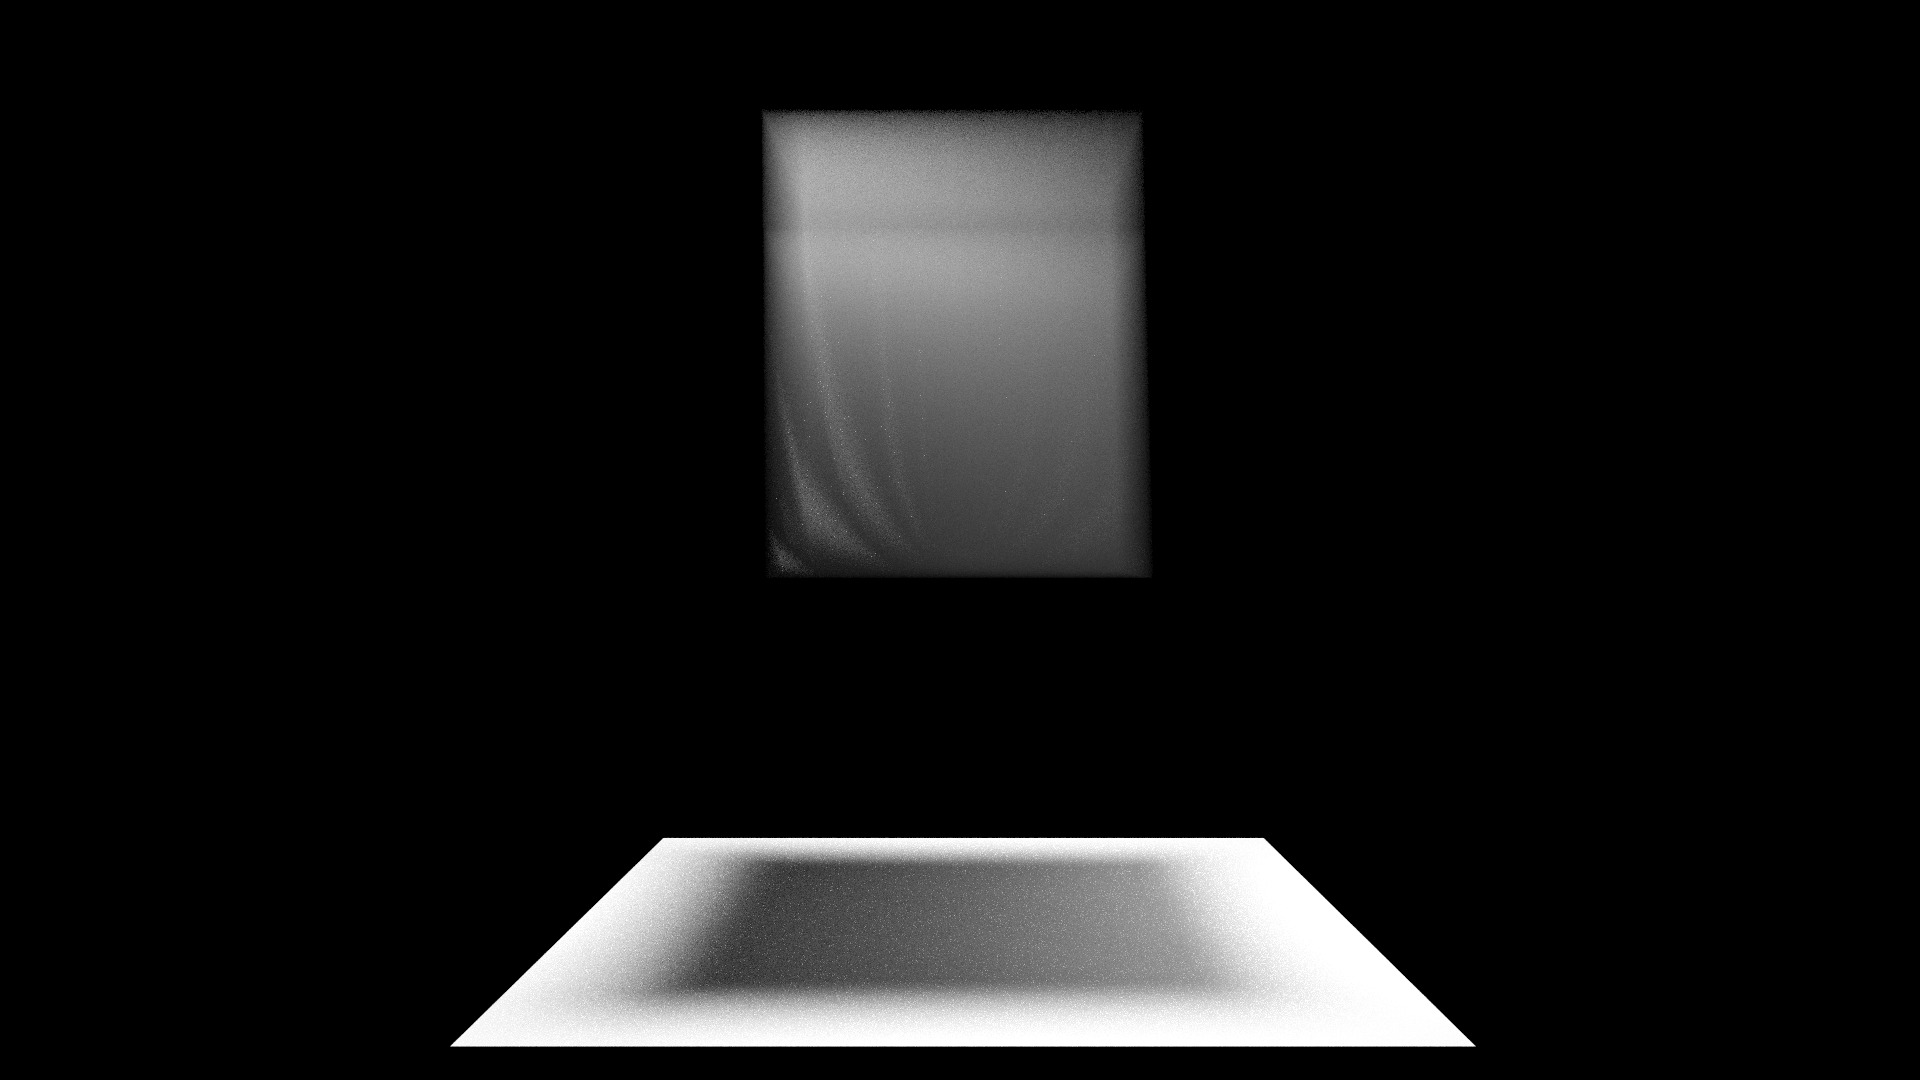
\includegraphics[width=\linewidth]{vol_shadow_inhomo}
	\caption{Inhomogeneous volumetric alpha shadow}
	\label{vol_alpha_inhomo}
\end{figure}

\subsubsection{Channel Independent Subsurface Scattering (BSSRDF)}

We have applied BSSRDF material to the \verb|Cornell Box| scene, resulting in the blue translucent box in \ref{bssrdf}.

\begin{figure}[h]
	\centering	
	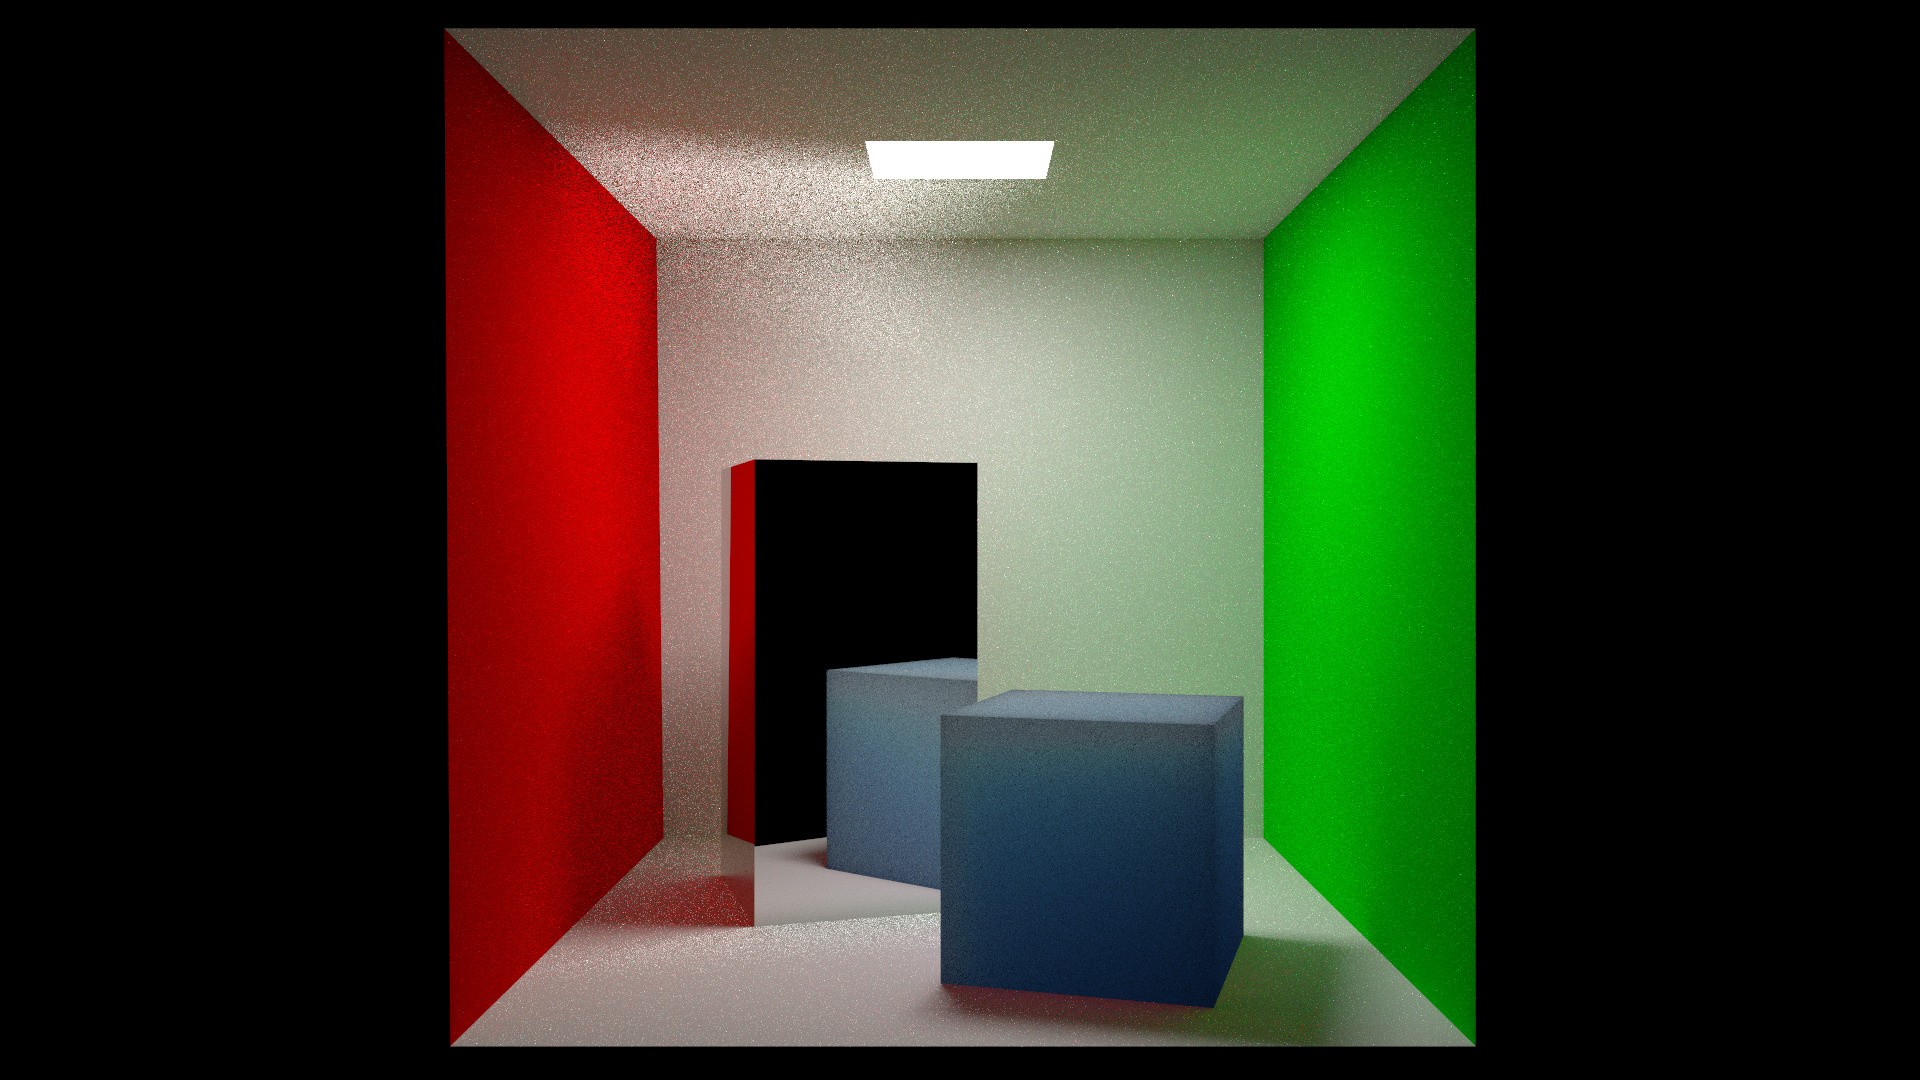
\includegraphics[width=\linewidth]{bssrdf}
	\caption{BSSRDF material}
	\label{bssrdf}
\end{figure}

\section{Functional Features}

\subsection{Texture Mapping}

We have implemented texture mapping and normal texture. \ref{color_texture} shows result of trivial color texture, while the fluctuation of sea surface (especially the reflection phenomenon) in \ref{sea} was acheived by normal texture. The corresponding raw texture is shown in \ref{noise}, which is generated by Perlin noise algorithm \cite{perlin_noise}.

\noindent \textbf{Contribution}: Shengquan Du; Noise generation done by Jingyi Lyu.

\begin{figure}[h]
	\centering	
	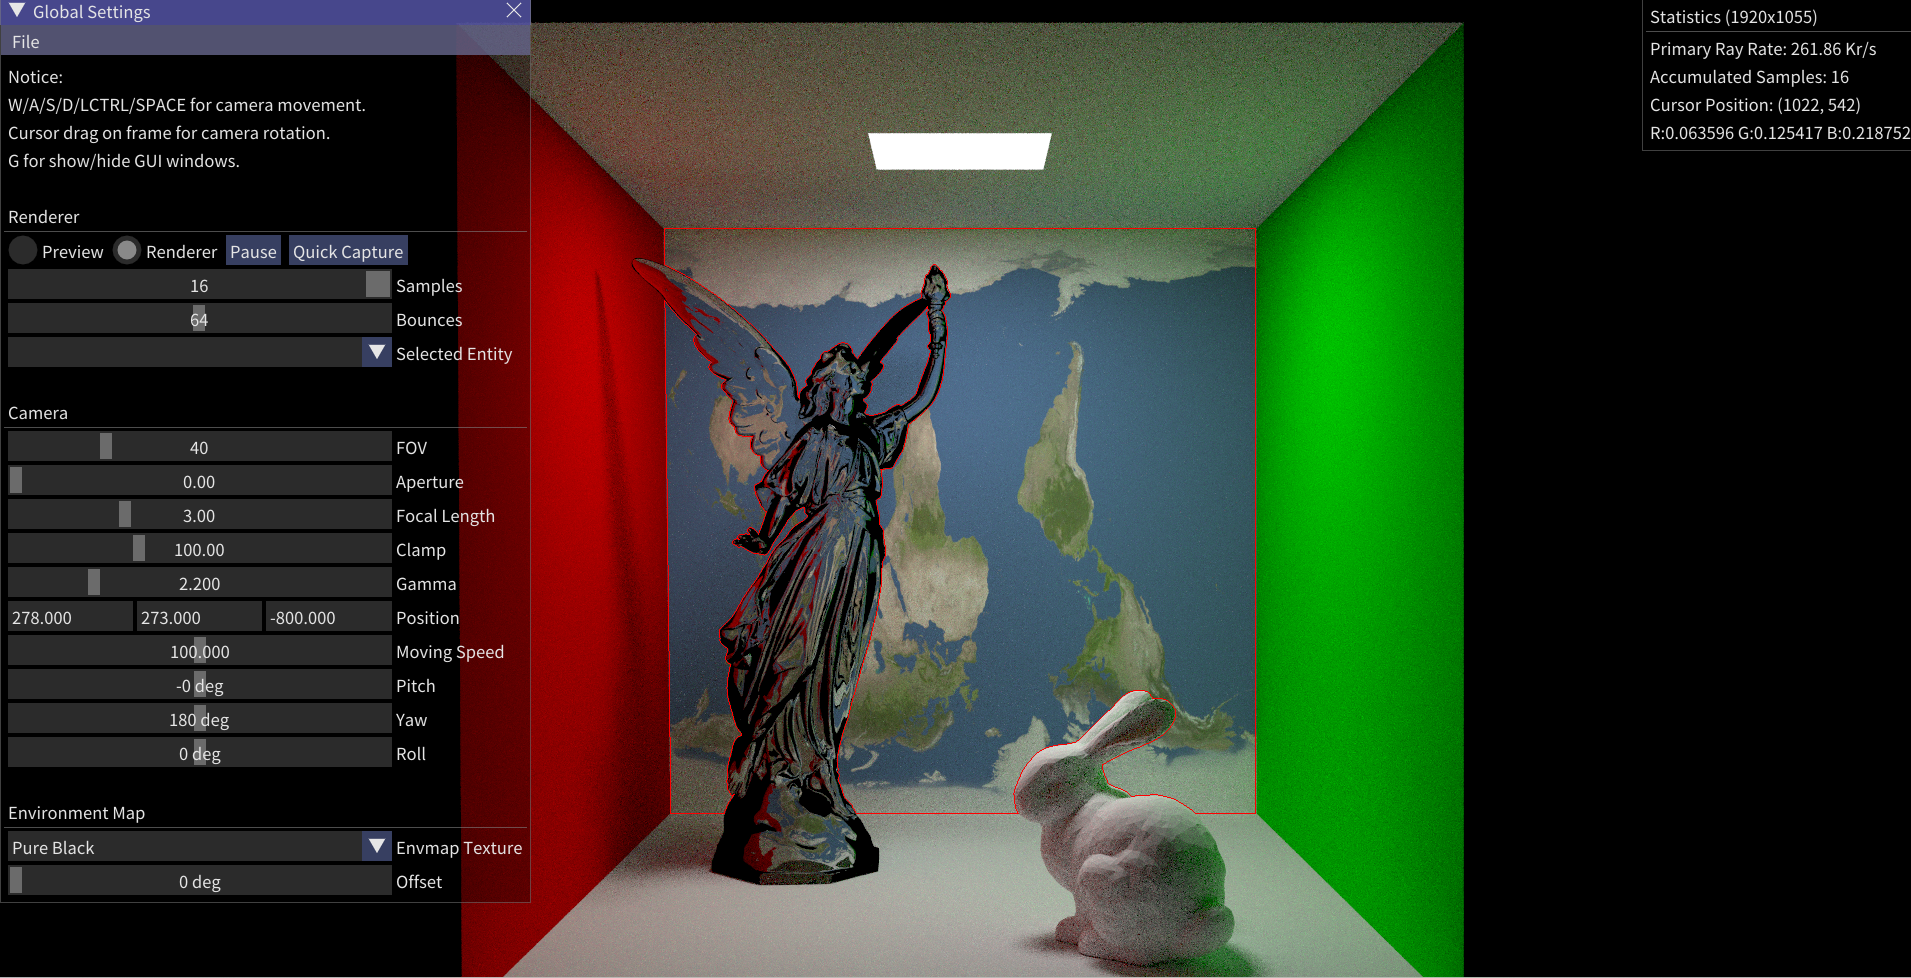
\includegraphics[width=\linewidth]{color_texture}
	\caption{Trivial color texture}
	\label{color_texture}
\end{figure}

\begin{figure}[h]
	\centering	
	
\includegraphics[width=\linewidth]{normal_noise_256}
	\caption{Raw perlin noise for normal texture}
	\label{noise}
\end{figure}

\subsection{Acceleration Structure}

We have implemented acceleration of intersection computation with BVH. Scene in \ref{color_texture} has thousands of triangles while the primary ray rate rendering it is still about $\frac{1}{3}$ of rendering \ref{cornell128}. 

\noindent \textbf{Contribution}: Shengquan Du.

\subsection{Importance Sampling}

Importance sampling and multiple importance sampling are applied to enhance path tracing convergence. The following figure \ref{mis} contains a typical setting for multiple importance sampling: Planes of different roughness reflecting light sources with different extent.

\noindent \textbf{Contribution}: Jingyi Lyu.

\begin{figure}[h]
	\centering	
	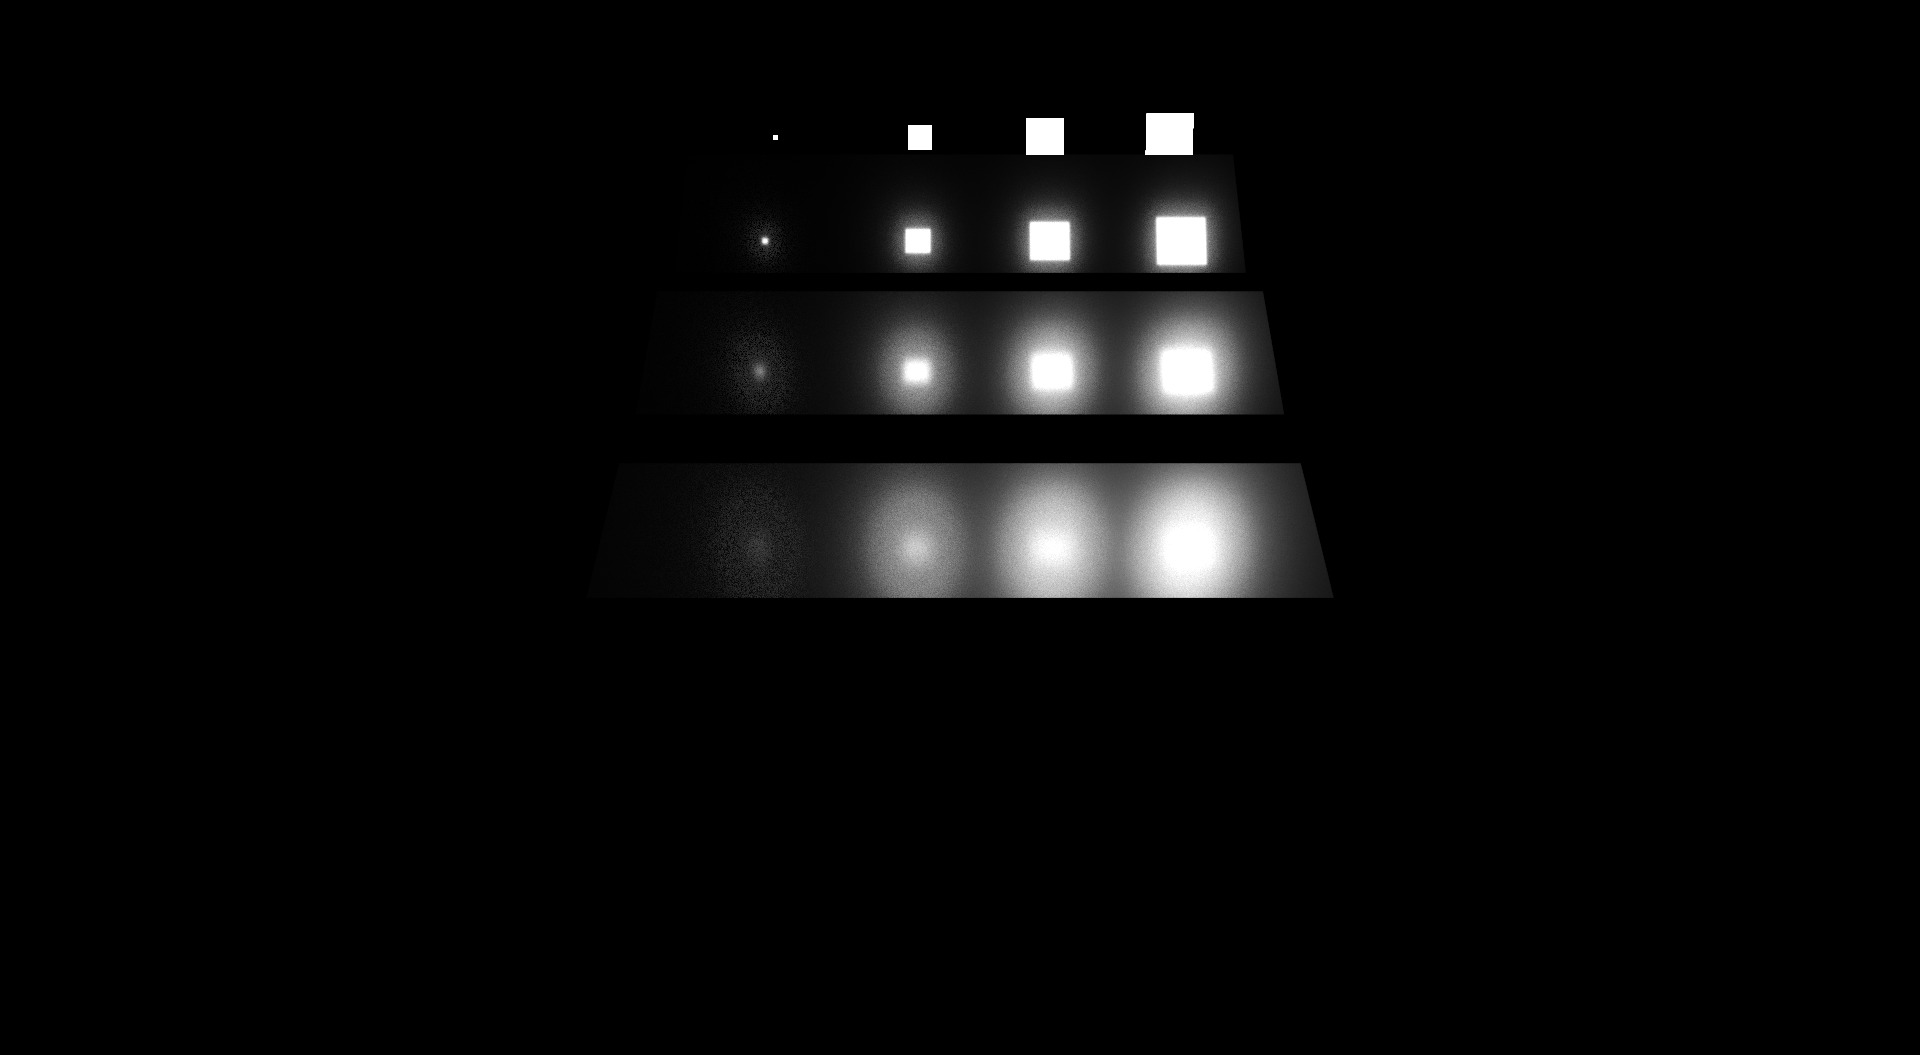
\includegraphics[width=\linewidth]{mis}
	\caption{Application of multiple importance sampling}
	\label{mis}
\end{figure}

\subsection{Anti-Aliasing}

Basic anti-aliasing by casting multiple rays through one pixel had been implemented by \verb|sparkium| framework, we just applied it throughout our rendering process.

\noindent \textbf{Contribution}: None.

\section{Special Visuial Effects}

\subsection{Depth Of Field}

Trivial aperture is also inherit function of camera in \verb|sparkium|. We applied it and obtained the following result in \ref{dof}.

\noindent \textbf{Contribution}: None.

\begin{figure}[h]
	\centering	
	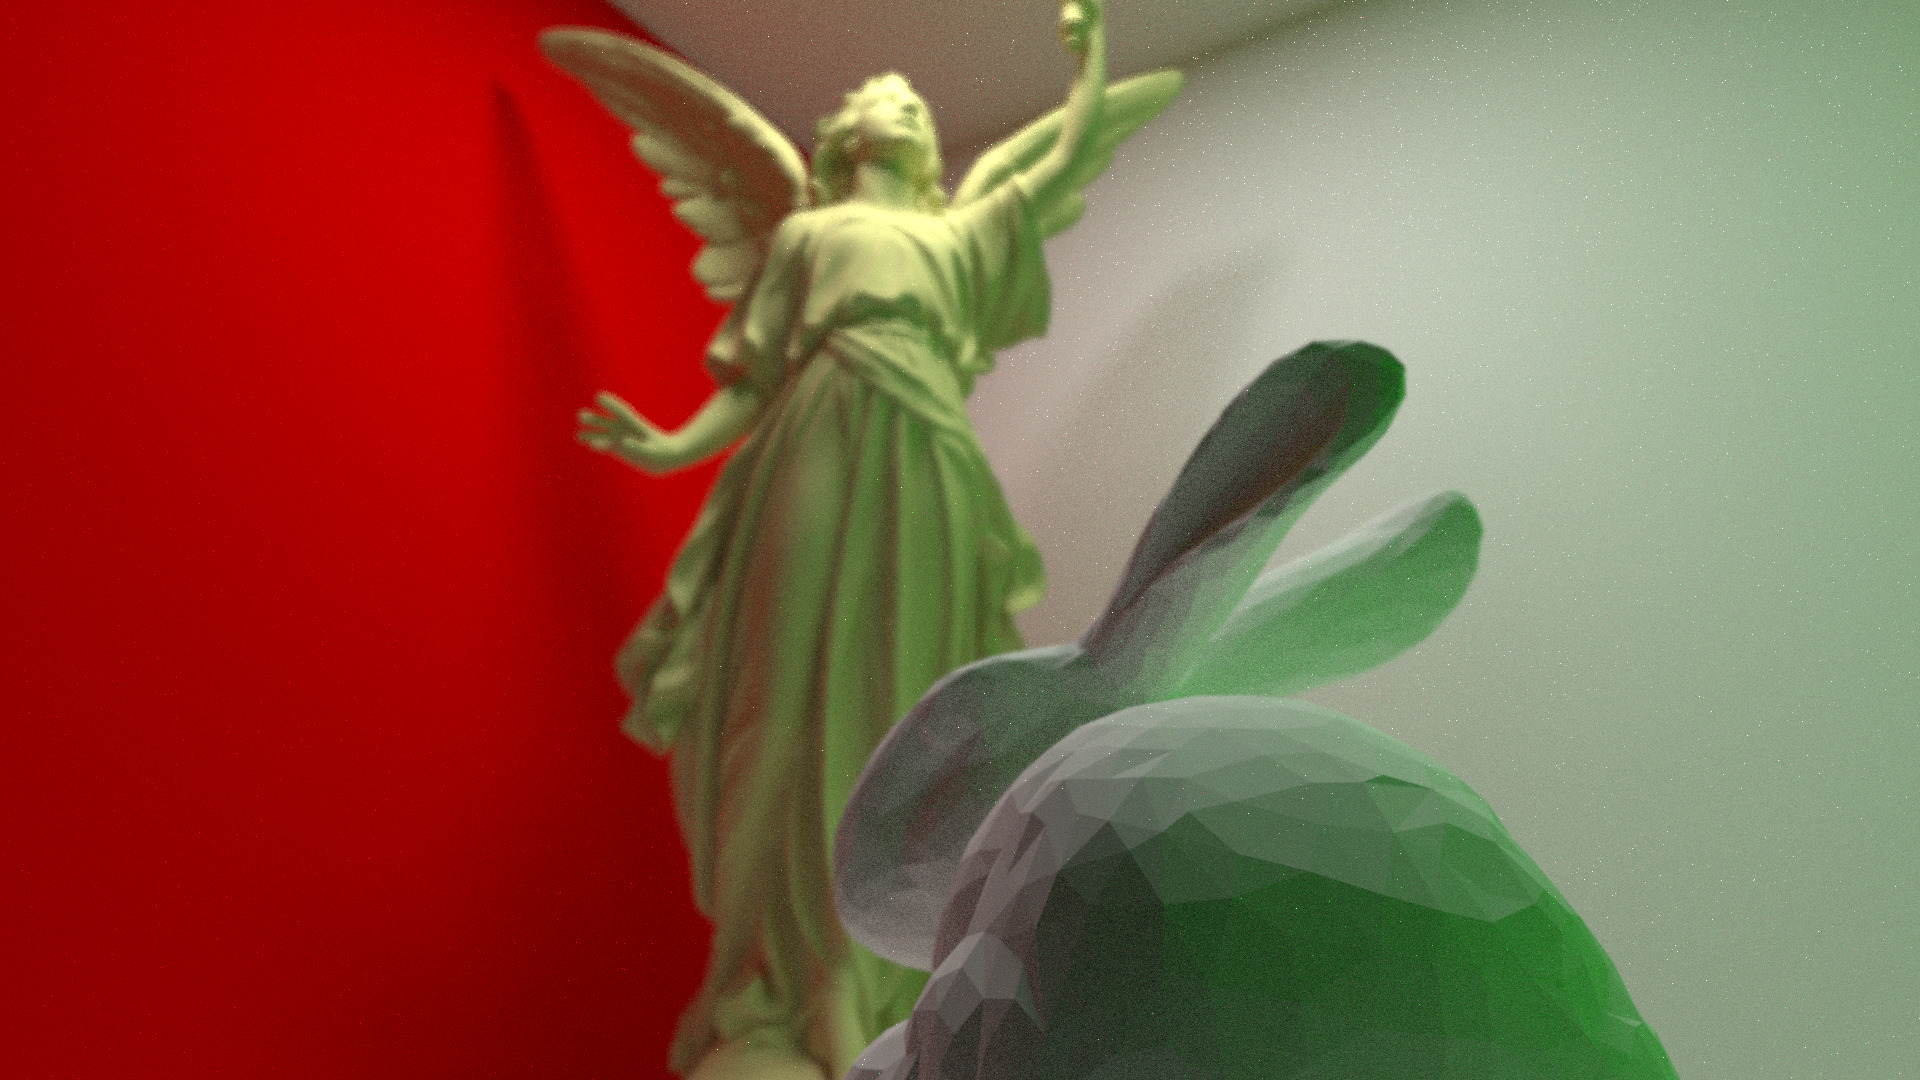
\includegraphics[width=\linewidth]{dof}
	\caption{Depth of field based on trivial aperture}
	\label{dof}
\end{figure}

\subsection{Motion Blur}

We have implemented motion blur effect and obtained the rotating Earth in \ref{motion_blur} as result.

\noindent \textbf{Contribution}: Shengquan Du.

\begin{figure}[h]
	\centering	
	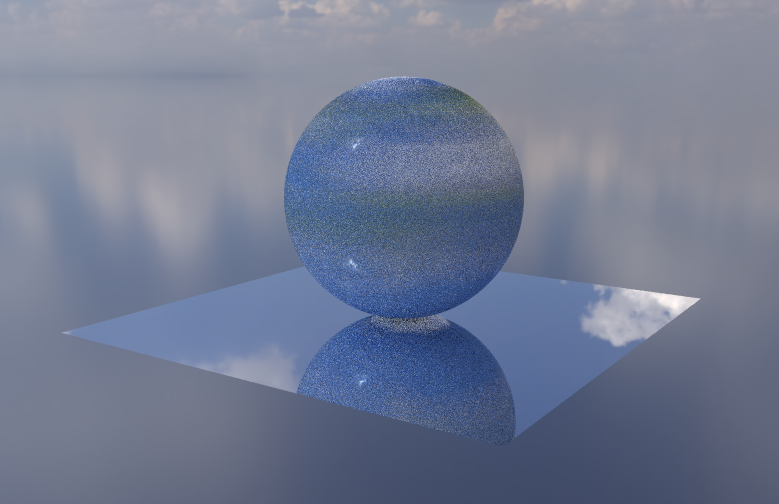
\includegraphics[width=\linewidth]{motion_blur}
	\caption{Motion blur: Earth rotating fast}
	\label{motion_blur}
\end{figure}

\section{Our Own Scene}

We collected 3D models from \cite{scene1}, \cite{scene2}, \cite{furina} and used Blender to manipulate and convert these models to meet the requirement of our framework and scene design. Then we applied various materials to those models, including principled BSDF (the character, sea and the throne), normal texture mapping (the see surface), volumetric fog (the beam and its scattering effect) and color texture (of the sky). The final result shown in \ref{my_scene} is an imitation of a CG appeared in Genshin Impact. 1920*1080 pixels and 256 samples per pixel are computed, costing 6 hours.

\noindent \textbf{Contribution}: Shengquan Du, Jingyi Lyu.

\begin{figure}[h]
	\centering	
	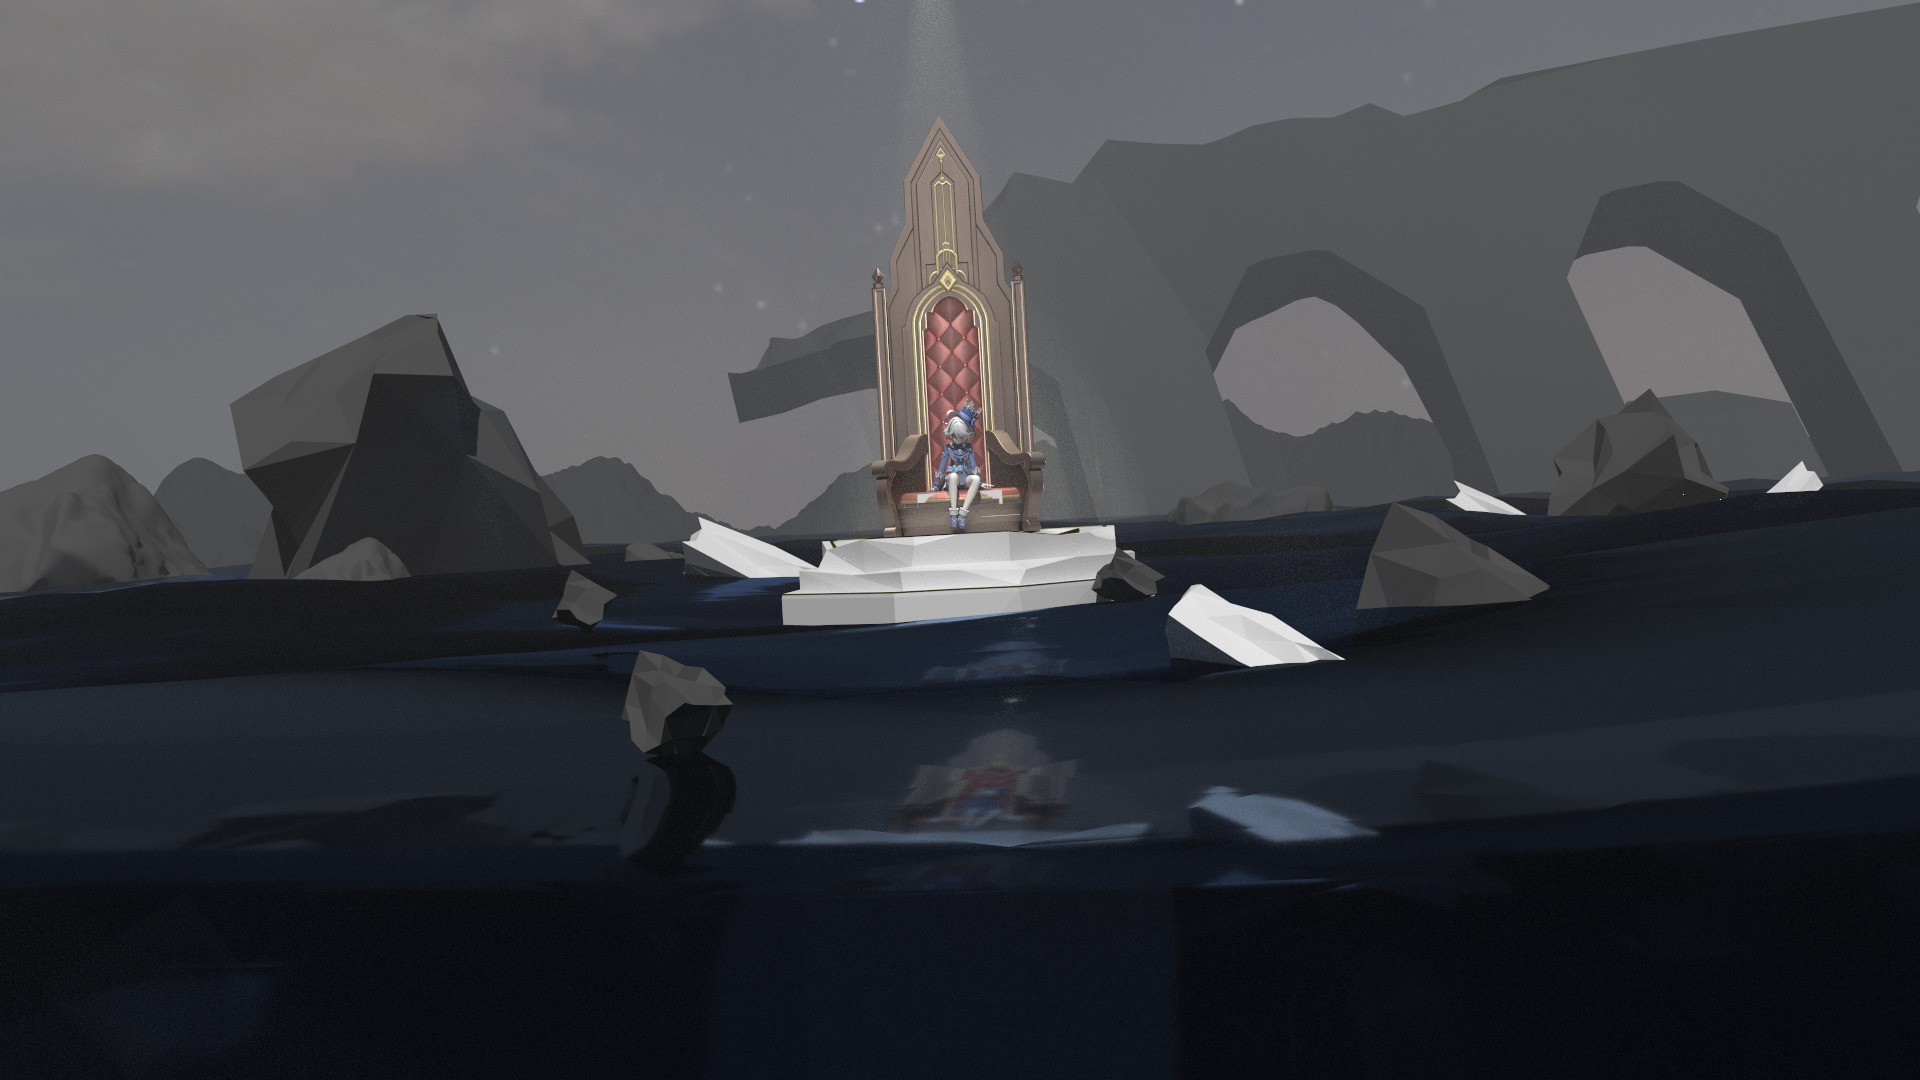
\includegraphics[width=\linewidth]{my_scene}
	\caption{Our final scene: Crisis of Fontaine prophecy}
	\label{my_scene}
\end{figure}

\section{Discussion}

We have noticed noisy light spot occurring sparsely during rendering process, which burdened convergence performance a lot since their strength are very large. We inferred that this could be caused by sampling incident direction near the top or edge of hemisphere. In this case, the sampling probability density could be very small, so the resulting incident illumination will be scaled tremendously. To tackle with this, we clamped all the probability density on denominator to $[p_l, +\infty)$, while all strength returned each recuresion to $[0, l_u]$, where $p_l, l_u$ are two parameters to adjust manually.

Apart from that, though the current render result is satisfying, we observed that behaviour of BSSRDF material is unstable sometimes, and its direct illumination may have some bugs. Since sampling and evaluation of BSSRDF are very complicated, we still need time to check them in the future.   

%%
%% The next two lines define the bibliography style to be used, and
%% the bibliography file.
\bibliographystyle{ACM-Reference-Format}
\bibliography{bib}

\end{document}
%%
%% End of file `sample-acmsmall-submission.tex'.
